\chapter{State of the art} % Main chapter title
\label{StateOfTheArt}

\section{Volume rendering algorithms}

The fundamental volume visualization algorithms described
below fall into two main categories: 

\begin{itemize}

\item Direct volume rendering (DVR) algorithms: they include approaches such as ray-casting, texture mapping, splatting, and V-buffer rendering. Splatting and V-buffer are also called projection methods. These these methods are characterized by mapping elements directly into screen space without using geometric primitives as an intermediate representation.

\item Surface-fitting (SF) algorithms : they are also called isosurfacing or feature-extraction. These algorithms consist in fitting surface primitives such as
polygons or patches to constant-value contour surfaces in volumetric datasets. The surface primitives used are most of the time planar.

\end{itemize}

DVR methods are especially appropriate for creating images from datasets containing amorphous features like clouds, fluids, and gases. One disadvantage of using DVR methods
is that the entire dataset must be traversed each time an image is
rendered. A low resolution pass or random sampling of the data is
sometimes used to create low-quality images quickly for parameter
checking. The process of successively increasing the resolution
and quality of a DVR image over time is called progressive
refinement.

 The user begins by choosing a threshold value
and then geometric primitives are automatically fit to the high-contrast
contours in the volume that match the threshold. Cells
whose comer-values are all above the chosen threshold (cell is
inside) or all below the threshold (cell is outside) are discarded and
have no effect on the final image. Showing just the cells falling on
the threshold is sometimes useful, but can be a problem. Another
consideration is the huge number of surface primitives generated
for large volumetric datasets. 


Many steps in the volume visualization process are common to
volume visualization algorithms.  Most of the fundamental volume
visualization algorithms include only a subset of the steps listed
here.
The initial step in every procedure is data acquisition. The next
common step is to pat the data slices into a form that can be worked
with and then to process each slice so that it covers a good
distribution of values, is high in contrast, and is free of noise and
out-of-range values. Of course, the same set of processes must be
applied to every slice.
Next, the dataset is reconstructed so that the ratio of the
dimensions is proportional to the ratio of the dimensions of the
measured substance or substance being simulated. This may
involve interpolating between values in adjacent slices to construct
new slices, replicating existing slices, interpolating to estimate
missing values, or scan-converting an irregular grid or nonorthogonal
grid onto a Cartesian grid by interpolation. At this point
three-dimensional enhancement may be applied, such as a slight
blurring of the data values. Next, a data-classification or
thresholding is performed. This step will be discussed in detail in
the section on data classification.
After data-classification, a mapping operation is applied to map
the elements into geometric or display primitives. This is the stage
that varies the most between algorithms, as will be shown in the
section on volume visualization algorithms. At this point the
primitives can be stored, manipulated, intermixed with externally
defined primitives, shaded, transformed to screen space, and
displayed. The shading and transformation steps can be reordered
and shading can be done in one of eleven ways as explained in 


\subsection{Direct Volume Rendering}

\subsubsection{Texture mapping}

\paragraph{2D Texture mapping}
2D Texture mapping consists in representing the whole volume as a set of slices parallel to coordinate planes. 
\begin{figure}[th]
\centering
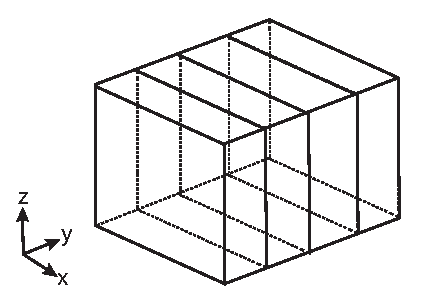
\includegraphics{Figures/2D_slices}
\decoRule
\caption[2D Sclices]{2D slices of the volume.}
\label{fig:2dslices}
\end{figure}

\subsubsection{Raycasting}


\subsection{Surface-fitting}

\section{Occlusion management strategies}

\subsection{Transfer Function}

\subsection{Segmentation}

\subsection{Deformations}

\section{Volume rendering in Virtual Reality and Augmented Reality}

\subsection{ Remote volume rendering}

Volumetric data exploration with direct volume rendering technique is of great help to visually extract relevant structures in many fields of science: medical imaging ~\cite{ljung_full_2006}, astrophysics and more recently in baggage inspection. To leverage this knowledge extraction, many techniques have been developed. 

In this section, we detail existing ones with volume visualization, transfer function, direct voxel manipulation, and focus plus context interaction.
Volume visualization can be done with geometric rendering system which transforms the data into a set of polygons representing an iso-surface. The contour tree algorithm ~\cite{carr_computing_2000} and other alternatives such as branch decomposition ~\cite{pascucci_multi-resolution_2004} are usually used to find these iso-surfaces. According to H. Guo ~\cite{guo_local_2013}, contour trees algorithms are vulnerable to noises, which can be problematic in baggage inspections since dense materials (e.g. iron) cause noises by reflecting the X-rays. For this reason we used the volume rendering technique; Chen et al. provide a review of existing techniques ~\cite{chen_3-d_2000}.
In order to investigate volumetric dataset, one can use the Transfer Function (TF). In practice, it maps the voxel density with a specific color (including its transparency). Transfer function can be 1D, 2D or nD and are of great help to isolate structures of interest in volumetric data ~\cite{kniss_multidimensional_2002}. Thanks to the color blending process, suitable transfer function can also reveal iso surface or hide density to improve the volumetric data visualization. The setup of this transfer function remains complex, but some automatic systems provide solution thanks to data analysis ~\cite{correa_size-based_2008} ~\cite{sereda_visualization_2006} ~\cite{patel_moment_2009} or user interactions ~\cite{guo_wysiwyg_2011}. Since our users have a limited knowledge on volume rendering, we developed new interaction techniques with sufficient abstraction level regarding technical constraints. These techniques will be detailed in this paper. As an example, we investigated predefined transfer functions with smooth transitions when changing their setup to reduce disruptive animation effects ~\cite{tversky_animation:_2002}.
Since graphic card power never stops to improve, new techniques allow the direct manipulation of the voxels which composes the volume to be displayed. Color tunneling introduced a set of interactions (lock, Brush, Dig) to explore 2D and 3D dataset composed of pixels of voxels ~\cite{hurter_interactive_2014} with point based rendering techniques ~\cite{sainz_point-based_2004} . Histomage also provides direct manipulation of pixels thanks to a histogram which can be used as a new selection and pixel modification tool ~\cite{chevalier_histomages:_2012}. Other interactive systems investigated pixel exploration with a lens as a focus plus context technique ~\cite{elmqvist_color_2011} ~\cite{hurter_moleview:_2011}. Our work provides additional interaction techniques with pixel based techniques ~\cite{hurter_interactive_2014} to address occlusion issues, focus and context awareness, reversibility of the actions, and continuity.  